\section{Introduction}

Current bathymetry measurement techniques range from physical collection performed by surface and sub-surface craft to mathematical computations based on satellite observation.  
There are applications where these methods fall short in that the satellite derived products do not produce the resolution needed and there are areas of the world where surveys cannot be conducted.  
To address this the Naval Research Laboratory (NRL) has proposed a research project titled “Predicting Global Altimetry” lead by geophysicist Dr. Warren Wood. 
The goal of this project is to develop models that will more accurately predict world-wide bathymetry values.  
The method being employed is to use machine learning to train algorithms to use different sets of input parameters, for different scenarios, to produce higher resolution bathymetry values.  
The input parameters these algorithms require come from multiple sources, but for the scope of this project we will focus on the ones that are calculated from existing datasets.  
It is NRL’s hypothesis that statistical and mathematically derived data from existing gridded bathymetric data sets can be used as input to increase prediction accuracy.

\begin{figure}[hb]
    \centering
    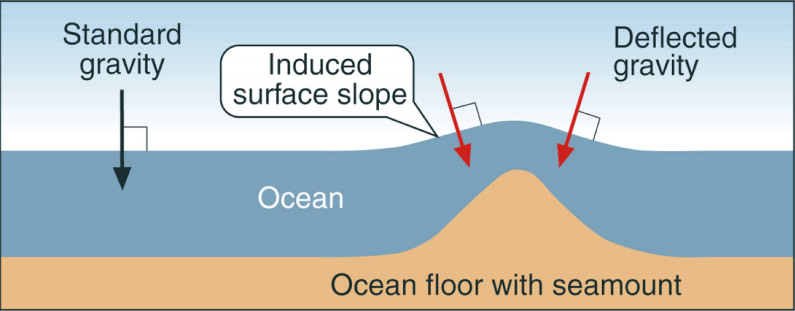
\includegraphics[scale=0.25]{mountainAltimetry}
    \caption{Graphic showing the Smith and Sandwell method}
    \label{fig1:Figure 2}
  \end{figure}

\par
Thw two main methods for predicting global bathymetry is the Smith and Sandwell method \cite{sandwell}, and ship soundings.
The Smith and Sandwell method uses satellite imagery to determine the mass of sea mounts.
That determined mass can then give a coarse prediction of the worlds bathymetry.
This technique is good for predicting bathymetry on a large coarse scale.
It does not preform well at predicting bathymetry for smaller portions of the globe.
Fine bathymetry measurements come from ship depth soundings.
These soundings give us the most accurate picture of the oceans topology.
However, preforming these ship soundings for the entire globe is costly, and impractical due to time constraints.